\documentclass {article}
\usepackage{caption}
\usepackage{datetime}
\usepackage{float}
\usepackage{amsmath}
\usepackage{eso-pic}
\usepackage{graphicx}
\usepackage{xcolor}
\usepackage{amssymb}
\usepackage{atbegshi,picture}
\usepackage{geometry}
\usepackage{ragged2e}
\usepackage[utf8]{inputenc}	
\geometry{a4paper,total={200mm,225mm},left=25mm,right=30mm}

\begin {document}

\begin{center}
	{\Large CHAPTER-7\\\vspace{0.2cm} TRIANGLES}
\end{center}
\AtBeginShipout{\AtBeginShipoutUpperLeft{%
	\put(\dimexpr\paperwidth-1cm\relax,-1.5cm){\makebox[0pt][r]{EXEMPLAR PROBLEMS}}%
}}

\textcolor{cyan}{\large EXERCISE 7.4}
\begin {enumerate}
\item Find all the angles of an equilateral triangle.
\item The image of an object placed at a point $A$ before a plane mirror $LM$ is seen at the point $B$ by an observer at $D$ as shown in Fig. 7.12. Prove that the image is as far behind the mirror as the object is in front  of the mirror.

[\textcolor{cyan}{Hint:} $CN$ is normal to the mirror. Also, angle of incidence = angle of reflection].
\begin{figure}[!h]
\centering
	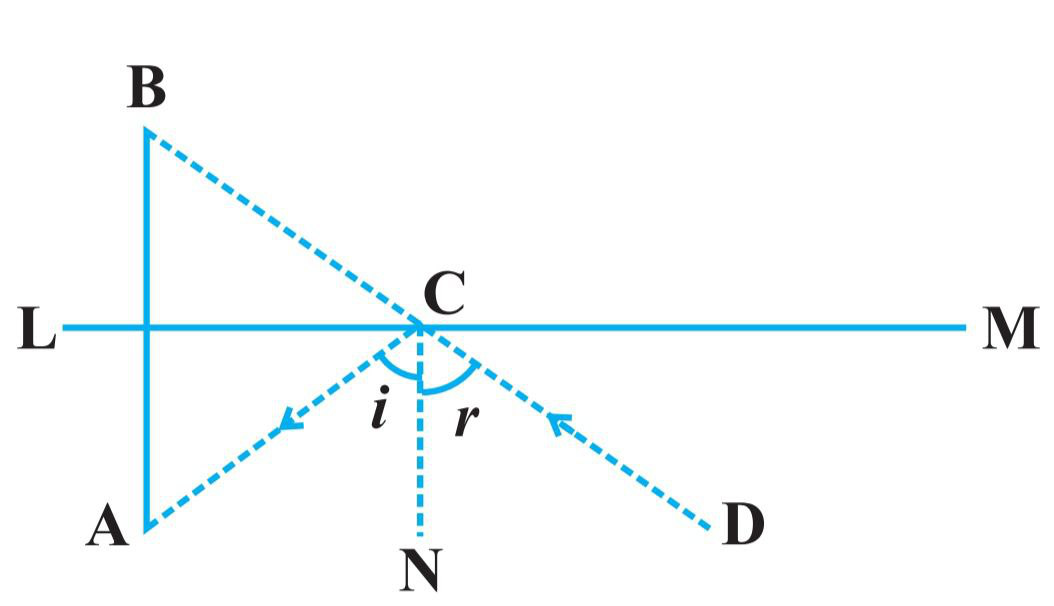
\includegraphics[scale=0.14]{./figs/7A.png}
\caption{Fig.7.12}
\label{fig:Fig.7.12}
\end{figure}
\item $ABC$ is an isosceles triangle with $AB = AC$ and $D$ is a point on $BC$ such that $AD\perp  BC$ (Fig. 7.13). To prove that $\angle BAD = \angle CAD$, a student proceeded as follows:\\
In $\triangle  ABD \text{ and }\triangle  ACD$,
\begin{align*}
AB &= AC &&\text{(Given)}\\
\angle B &= \angle C &&\text{(because $AB = AC$)}\\
\text{ and }
\angle ADB &= \angle ADC\\
\therefore \triangle  ABD &\cong  \triangle ACD &&\text {(AAS)} \\
\text { So, }  \angle BAD &= \angle CAD &&\text{(CPCT)}
\end{align*}
What is the defect in the above arguments?

[\textcolor{cyan}{Hint:} Recall how $\angle B = \angle C $ is proved when $AB = AC$].
\begin{figure}[!h]
\centering
	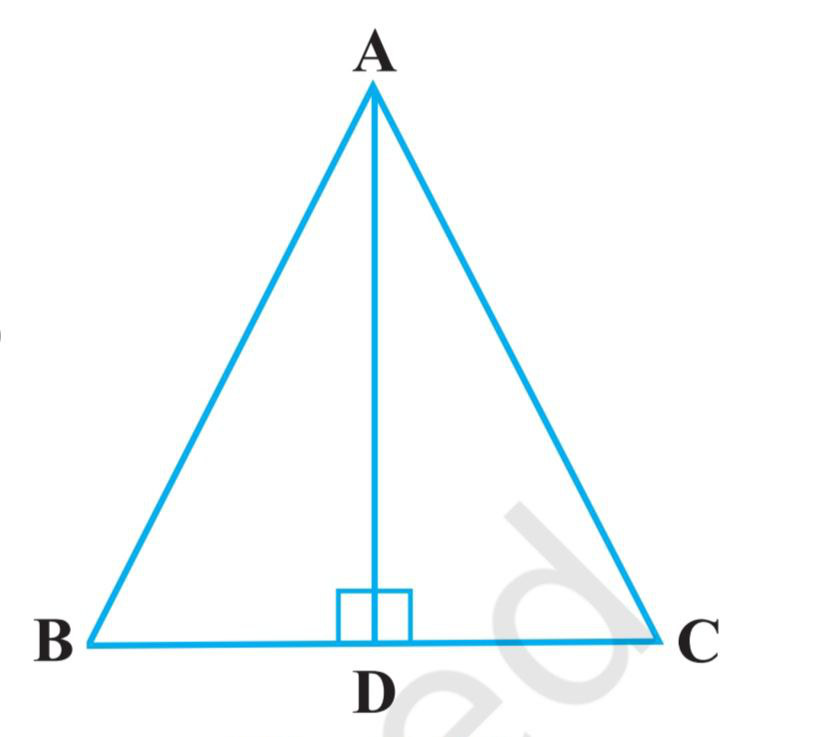
\includegraphics[scale=0.14]{./figs/7B.png}
\caption{Fig.7.13}
\label{fig:Fig.7.13}
\end{figure}
\item $P$ is a point on the bisector of $\angle ABC$. If the line through $P$, parallel to $BA$ meet $BC$ at $Q$, prove that $BPQ$ is an isosceles triangle.
\item $ABCD$ is a quadrilateral in which $AB = BC$ and $AD = CD$. Show that $BD$ bisects both the angles $ABC$ and $ADC$.
\item $ABC$ is a right triangle with $AB = AC$. Bisector of $\angle A$ meets $BC$ at $D$. Prove that $BC = 2 AD$
\item $O$ is a point in the interior of a square $ABCD$ suchthat $OAB$ is an equilateral triangle. Show that $\triangle  OCD$ is an isosceles triangle.
\item $ABC$ and $DBC$ are two triangles on the same base $BC$ such that $A$ and $D$ lie on the opposite sides of $BC$, $AB = AC$ and $DB = DC$. Show that $AD$ is the perpendicular bisector of BC.
\item ABC is an isosceles triangle in which $AC = BC$. $AD$ and $BE$ are respectively two altitudes to sides $BC$ and $AC$. Prove that $AE = BD$.
\item Prove that sum of any two sides of a triangle is greater than twice the median with respect to the third side.
\item Show that in a quadrilateral $ABCD$, 
\begin{align*}
     AB + BC + CD + DA  <  (BD + AC)
\end{align*}	
\item Show that in a quadrilateral $ABCD$,
\begin{align*}
	AB + BC + CD + DA  >   AC + BD
\end{align*}
\item In a triangle $ABC$, $D$ is the mid-point of side $AC$ such that $ BD = \frac{1}{2} AC $. Show that $\angle ABC$ is a right angle.
\item In a right triangle, prove that the line-segment joining the mid-point of the hypotenuse to the opposite vertex is half the hypotenuse.
\item Two lines $l$ and $m$ intersect at the point $O$ and $P$ is a point on a line $n$ passing through the point $O$ such that $P$ is equidistant from $l$ and $m$. Prove that $n$ is the bisector of the angle formed by $l$ and $m$.
\item Line segment joining the mid-points $M$ and $N$ of parallel sides $AB$ and $DC$, respectively of a trapezium $ABCD$ is perpendicular to both the sides $AB$ and $DC$. Prove that $AD = BC$.
\item $ABCD$ is a quadrilateral such that diagonal $AC$ bisects the angles $A$ and $C$. Prove that $AB = AD$ and $CB = CD$.
\item $ABC$ is a right triangle such that $AB = AC$ and bisector of angle $C$ intersects the side $AB$ at $D$. Prove that $AC + AD = BC$.
\item $AB$ and $CD$ are the smallest and largest sides of a quadrilateral $ABCD$. Out of $\angle B$ and $\angle D$ decide which is greater.
\item Prove that in a triangle, other than an equilateral triangle, angle opposite the longest side is greater than $\frac{2}{3}$ of a right angle.
\item $ABCD$ is quadrilateral such that $AB = AD$ and $CB = CD$. Prove that $AC$ is the perpendicular bisector of $BD$.
\end{enumerate}
\end{document}
